% Summary Report Senior Chemistry Template
% by Lydia Drabsch
% Created 8/8/15
\documentclass[12pt,a4paper]{article}
\usepackage[top=2cm, bottom=2cm, left=2cm, right=2cm]{geometry}
%\usepackage{rsc}
\bibliographystyle{IEEEtran}

% Figure packages
\usepackage{chngcntr}
\usepackage{tikz}
\usepackage{graphicx}
%\counterwithin{figure}{section}
\usepackage{epigraph}
%\usepackage{subfigure}
\usepackage{epstopdf}
\usepackage{epsfig}
\DeclareGraphicsExtensions{.eps}
\setlength{\intextsep}{5pt plus 1.0pt minus 1.0pt}
	
% Table Packages
\usepackage{multirow}
%\counterwithin{table}{section}
\usepackage{booktabs}
\usepackage{multicol}

% Formatting packages
\usepackage{hyperref}
\usepackage{chngcntr}
\usepackage{indentfirst}    %remove if we dont want to indent
\hypersetup
	{
		colorlinks,%
		citecolor=black,%
		linkcolor=black,%
		urlcolor=black,%
	}
\newcommand{\temp}{$^{\circ}$C }
\newcommand{\gm}{g mol$^{-1}$ }
\newcommand{\Mgm}{g\;mol^{-1}}

% titles packages
\usepackage{titlesec}
\setcounter{tocdepth}{5}
\usepackage{caption}
\usepackage{subcaption}
\setcounter{secnumdepth}{5}
\usepackage{color}
\definecolor{titlecolour}{cmyk}{1,.1,0.0,.50}
\definecolor{scolour}{cmyk}{1,.0,0,.3}
\definecolor{sscolour}{cmyk}{1,.0,0.0,.75}
\definecolor{ssscolour}{cmyk}{1,.0,0.0,.65}
\definecolor{paracolour}{cmyk}{1,.0,0.0,.55}

\usepackage{titlesec}
\usepackage{bold-extra}
%\titleformat{\maketitle}{\color{titlecolour}}{}{}{}
\titleformat{\section}
{\color{scolour}\scshape\Large\bfseries}
{\color{scolour}\thesection}{1em}{}
\titleformat{\subsection}
{\color{sscolour}\normalfont\bfseries}
{\color{sscolour}\thesubsection}{2em}{}
%\titleformat{\subsubsection}
%{\color{ssscolour}\normalfont\Large\bfseries}
%{\color{ssscolour}\thesubsubsection}{3em}{}
%\titleformat{\paragraph}
%{\color{paracolour}\normalfont\large\bfseries}
%{\color{paracolour}\theparagraph}{4em}{}
\titlespacing\section{0pt}{12pt plus 4pt minus 2pt}{0pt plus 2pt minus 2pt}
\titlespacing\subsection{0pt}{10pt plus 4pt minus 2pt}{0pt plus 2pt minus 2pt}


% maths packages
\usepackage{amsmath}
\usepackage{amsfonts}
\usepackage{amssymb}



\newcommand{\degs}{$^{\circ}$C }

% magnetosphere - 

\begin{document}
\newgeometry{top=2cm, bottom=2cm, left=1.5cm, right=1.5cm}
{\centering\bf\LARGE\color{titlecolour} Mini Magnetosphere: Active Spacecraft Shielding from the Van Allen Belts    \par} % in geocentric orbits
{\centering\bf Lydia Drabsch\par}
{\bf\centering 12th April 2016\par}



\section*{Background}
The Van Allen belts are regions of trapped charged particles that encompass the Earth ranging from 1000 km to 60000 km from the surface of the Earth. Typically there are two belts with the inner belt mostly comprised of protons and an outer belt mostly containing electrons. Except for very Low Earth Orbits, spacecraft require shielding from the charged particles to prevent single-event effects on the electronics \cite{VanAllen}. Components are also radiation hardened before launch, which increases the cost of spacecraft manufacture. The most widely used form of shielding is passive shielding, where masses of material is used to absorb the radiation. However, this increases the mass of the spacecraft which in turn increases the cost of launch.\\

The environment inside the Van Allen belts have been investigated by NASA's Radiation Belt Storm Probes twin satellites. One of the primary mission objectives is to develop empirical and physical models predicting radiation belt space weather effects \cite{RBSP}. This data will be used to model the incident plasma that the device will shield against.\\

 % difficulty?
A different form of shielding called active shielding is another option for spacecraft. Previous methods of active shielding include electrostatic fields, plasma shielding, confined and unconfined magnetic fields to deflect the charged particles from the spacecraft \cite{townsend}.\\

Active shielding has been difficult in the past because the charged particles are very high in energy. This requires high voltages to be able to deflect the particles, or to deflect them over a long distance \cite{mainweb}. Low temperature superconductors to generate high magnetic fields have been explored \cite{magthesis}, however the extra mass of the ma
Some theoretical models would require kilometers in diameter charged surfaces to deflect the particles \cite{townsend}. The shield also needs to deflect both positive and negative charge without accumulating a charge build up \cite{PlasmaRadShielding}. The shielding device also needs to not interfere with the communication, propulsion and power generation of the spacecraft, or provide solutions as to how they can be interfaced. Other difficulties include the need for a reliable and stable device that can operate for the lifetime of the spacecraft without intervention. 


% idea: have some way to collect the ions  - magnetic field - magnetic mirror - collect them at the apex with a small voltage - use a propulsion?
\vspace{12pt}
\hrule
\vspace{3mm}
%\vspace{-10pt}
\noindent\textbf{\scshape\Large\color{scolour}Problem Statement:} Investigate, design and verify an active shielding configuration for spacecraft from plasma effects present in the Van Allen Belts. 
\vspace{3mm}
\hrule



\section*{Method of Attack}
\begin{enumerate}
\item Identify the design constraints required of a spacecraft. Constraints include dimensions, power requirements, mass and minimal communication interference.
\item Design three different magnetic field configurations with the guidance of previous and theoretical designs. The first configuration will be only a magnetic field shield. The second configuration will incorporate a plasma contained by a magnetic field. The third configuration will be based on a purely theoretical design of an inflating magnetic field.
\item Simulate the design configurations in COMSOL Multiphysics and identify the required strength of the magnetic field in order to shield the spacecraft. 
\item Only one configuration will be built and tested. Resource accessibility will influence the decision as well as the simulation models.
\item The chosen configuration will be built as well as the incident plasma and sensors.
\item The prototype will be tested to verify the simulation models.
\item A potential expansion could be to create a feedback control system in MATLAB to interface with COMSOL to model incident plasma fluctuations. These fluctuations occur during solar storms and greatly influence the space weather.  
\end{enumerate}

\begin{figure}[h]
\centering
\caption{Thesis Breakdown and Schedule}
\label{fig:ProposalGantt}
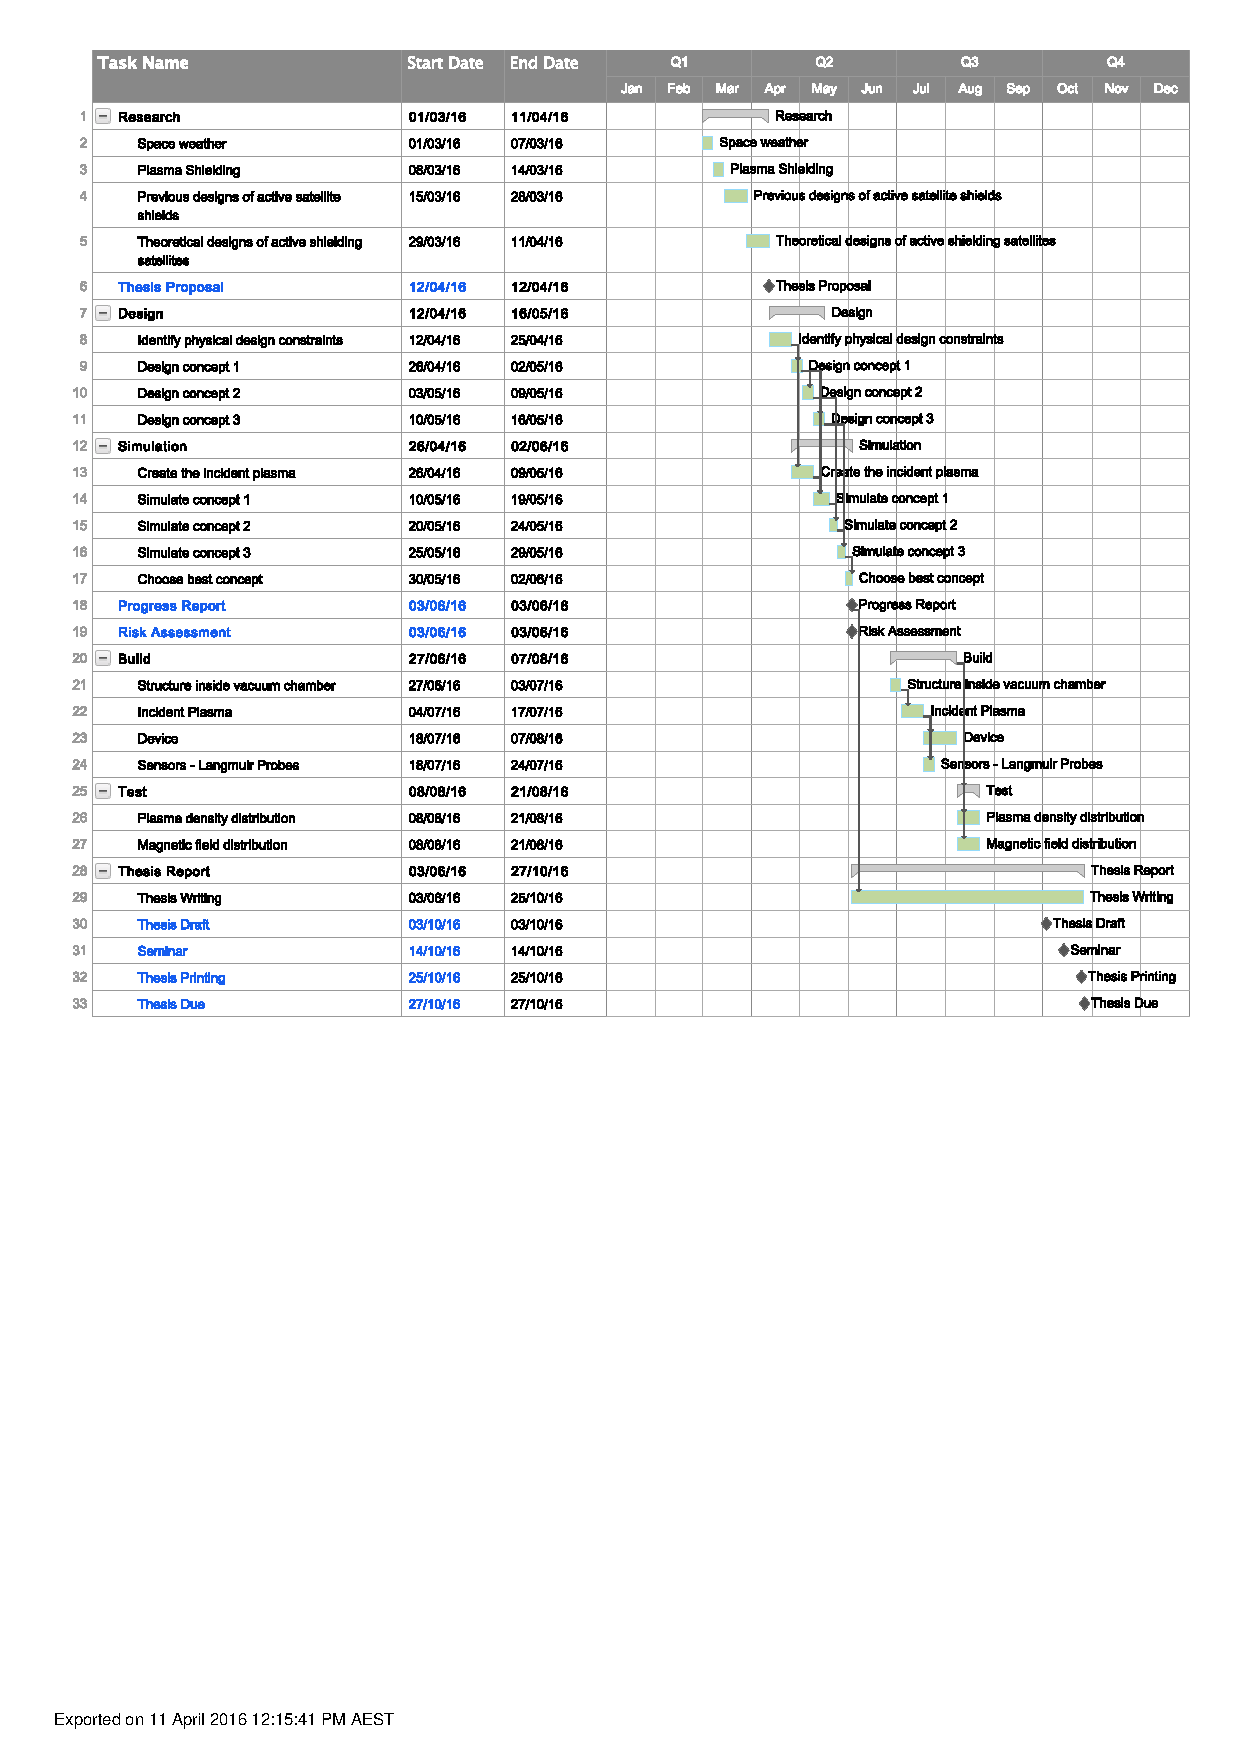
\includegraphics[trim = 1cm 12.2cm 0 8mm, clip,width=1\linewidth]{ProposalGantt.pdf}
\end{figure}



\section*{Resource Plan}

The School of Physics at the University of Sydney has equipment that is available to access including a vacuum chamber and high voltage sources. Most experimental work will be done at the School of Physics Laboratory where general resources are available such as copper wire for electromagnetic coils. 



%\section*{Risk Management}
%High voltage devices will be used to generate the magnetic field, 






\bibliography{proposal_bib}{}
\bibliographystyle{alphadin}
%\section{References}
%\url{https://engineering.dartmouth.edu/~d76205x/research/Shielding/docs/Seth_Watkins_Duke_1993.pdf} \\
%\url{http://engineering.dartmouth.edu/~d76205x/research/Shielding/docs/ToMaSS.pdf}






\end{document}

